\section{Задание 3. Осциллятор}

\subsection{Постановка и общий анализ}

Исследуется система $\dot x=Ax$:

\begin{equation}
\dot x_1=x_2,\qquad \dot x_2=ax_1+bx_2,\qquad
A=\begin{pmatrix}0&1\\a&b\end{pmatrix}.
\end{equation}

Второе уравнение эквивалентно $\ddot x_1-b\dot x_1-ax_1=0$. Характеристический многочлен и собственные числа:

\begin{equation}
\det(\lambda I-A)=\lambda^2-b\lambda-a,\qquad
\lambda_{1,2}=\frac{b\pm\sqrt{b^2+4a}}{2}.
\end{equation}

Из первой строки $(A-\lambda I)v=0$ получаем $v_2=\lambda v_1$. Поэтому для любого корня можно взять $v(\lambda)=(1,\lambda)^T$. При разных корнях общее решение равно

\begin{equation}
x(t)=c_1e^{\lambda_1t}\begin{pmatrix}1\\\lambda_1\end{pmatrix}
+c_2e^{\lambda_2t}\begin{pmatrix}1\\\lambda_2\end{pmatrix},
\end{equation}

\begin{equation}
c_1=\frac{x_2(0)-\lambda_2x_1(0)}{\lambda_1-\lambda_2},\quad
c_2=\frac{\lambda_1x_1(0)-x_2(0)}{\lambda_1-\lambda_2}.
\end{equation}

Для вещественной матрицы комплексные моды берутся в сопряжённых парах, что даёт вещественное решение. Если оба собственных числа имеют отрицательные вещественные части, нулевое равновесие асимптотически устойчиво. Наличие положительной вещественной части даёт неустойчивость. Чисто мнимые различные корни в рассматриваемой системе дают устойчивый центр, без стремления к нулю.

\subsection{Физическая модель и начальные условия}

Все четыре случая реализуются одним типом реальной системы: математический маятник с вязким сопротивлением в шарнире, рассматриваемый около нижнего либо верхнего положения равновесия. Груз массы $m$ закреплён на лёгком жёстком стержне длины $l$. Для верхнего положения нужен именно стержень, способный удерживать груз над шарниром. Угол $\theta$ отсчитывается от соответствующего равновесия; момент сопротивления равен $-c\dot\theta$, где $c\geq0$.

Моменты сил относительно шарнира дают около нижнего положения

\begin{equation}
ml^2\ddot\theta=-mgl\sin\theta-c\dot\theta,
\end{equation}

а около верхнего положения при таком же выборе положительного направления угла

\begin{equation}
ml^2\ddot\theta=+mgl\sin\theta-c\dot\theta.
\end{equation}

Для малых углов $\sin\theta\approx\theta$. После деления на $ml^2$ получаем исследуемую систему:

\begin{equation}
x_1=\theta,\qquad x_2=\dot\theta,\qquad
a=\begin{cases}-g/l,&\text{нижнее положение},\\+g/l,&\text{верхнее положение},\end{cases}
\qquad b=-\frac{c}{ml^2}.
\end{equation}

Переменная $x_1$ — угловое отклонение в радианах, $x_2$ — угловая скорость в радианах в секунду. Параметр $a$ имеет размерность $\mathrm{с}^{-2}$ и задаёт возвращающее либо опрокидывающее действие тяжести; $b$ имеет размерность $\mathrm{с}^{-1}$ и задаёт вязкое затухание. При $b=0$ сопротивлением пренебрегаем.

Берём $g=9{,}81\ \mathrm{м/с^2}$, $l=g/4=2{,}4525\ \mathrm{м}$, $m=1\ \mathrm{кг}$. Тогда $a=\pm4$. Значения $b=-2,-3,-4,-5$ реализуются коэффициентами $c=2ml^2,3ml^2,4ml^2,5ml^2$ соответственно, в $\mathrm{Н\cdot м\cdot с}$.

Для всех основных графиков выбраны одинаковые пять ненулевых начальных состояний:

\begin{equation}
\begin{gathered}
x^{(1)}(0)=\begin{pmatrix}0{,}08\\0\end{pmatrix},\quad
x^{(2)}(0)=\begin{pmatrix}0\\0{,}16\end{pmatrix},\quad
x^{(3)}(0)=\begin{pmatrix}-0{,}08\\0{,}08\end{pmatrix},\\[6pt]
x^{(4)}(0)=\begin{pmatrix}0{,}08\\-0{,}16\end{pmatrix},\quad
x^{(5)}(0)=\begin{pmatrix}0{,}04\\-0{,}16\end{pmatrix}.
\end{gathered}
\end{equation}

В неустойчивых случаях общие траектории линейной модели показаны до $t=2\ \mathrm{с}$; для устойчивых выбран интервал $0\leq t\leq8\ \mathrm{с}$. Устойчивые ветви седла дополнительно показаны отдельно до $4\ \mathrm{с}$, чтобы они не терялись на фоне растущих решений. Точки на фазовых кривых обозначают начальные состояния, стрелки — направление времени.

Линейная модель описывает реальный маятник только при малых углах. Растущие решения после выхода из малой окрестности равновесия показывают свойства линейной системы; они не означают неограниченного физического роста угла по тому же закону. Для вывода о локальной неустойчивости достаточно начального ухода из окрестности.

\subsection{Случай 1. a < 0, b = 0}

\textbf{Модель.} Маятник около нижнего положения, сопротивление отсутствует. Выбираем $a=-4$, $b=0$:

\begin{equation}
A_1=\begin{pmatrix}0&1\\-4&0\end{pmatrix},\qquad
\lambda^2+4=0,\qquad \lambda_{1,2}=\pm2i.
\end{equation}

Собственные векторы $v_+=(1,2i)^T$, $v_-=(1,-2i)^T$. Обобщённые собственные векторы не нужны: корни различные. Вещественных собственных направлений нет.

Для $q=x_1(0)$, $u=x_2(0)$ решение имеет вид

\begin{equation}
x_1(t)=q\cos(2t)+\frac{u}{2}\sin(2t),\qquad
x_2(t)=-2q\sin(2t)+u\cos(2t).
\end{equation}

Период $T=\pi\ \mathrm{с}$. Величина $H=(x_2^2+4x_1^2)/2$ сохраняется, поэтому фазовые кривые — эллипсы $x_2^2+4x_1^2=\mathrm{const}$. В точке $x_1>0,x_2=0$ поле направлено вниз, следовательно, обход эллипсов идёт по часовой стрелке.

На рисунках \ref{fig:t3_1_x1}, \ref{fig:t3_1_x2}, \ref{fig:t3_1_phase} показаны незатухающие периодические движения и замкнутые фазовые кривые.

\begin{figure}[H]\centering
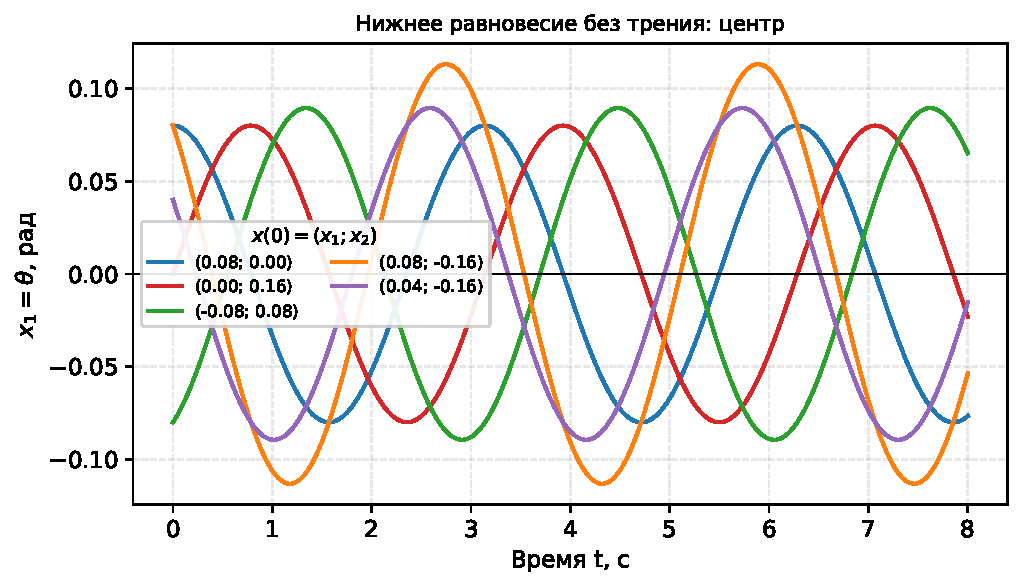
\includegraphics[width=0.82\linewidth]{../figures/t3_1_x1.pdf}
\caption{Угловое отклонение маятника без сопротивления около нижнего положения}\label{fig:t3_1_x1}
\end{figure}

\begin{figure}[H]\centering
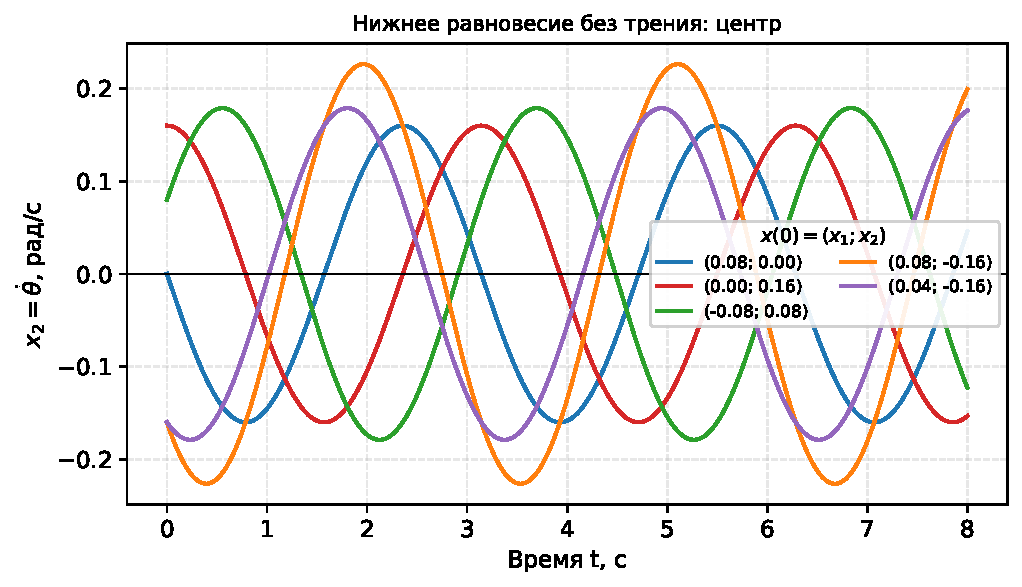
\includegraphics[width=0.82\linewidth]{../figures/t3_1_x2.pdf}
\caption{Угловая скорость маятника без сопротивления около нижнего положения}\label{fig:t3_1_x2}
\end{figure}

\begin{figure}[H]\centering
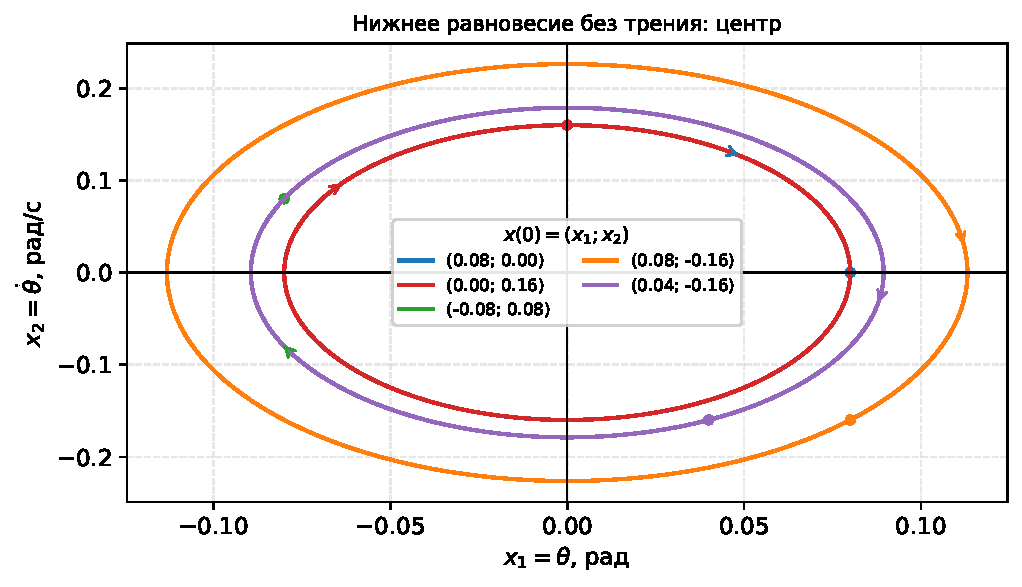
\includegraphics[width=0.82\linewidth]{../figures/t3_1_phase.pdf}
\caption{Фазовые траектории: центр, незатухающие колебания}\label{fig:t3_1_phase}
\end{figure}

\textbf{Вывод.} Нулевое равновесие устойчиво по Ляпунову, но не асимптотически устойчиво. Сколь угодно малое начальное отклонение остаётся малым, однако ненулевое решение не стремится к нулю, поскольку энергия сохраняется. Тип портрета — центр.

\subsection{Случай 2. a < 0, b < 0}

\textbf{Модель.} Маятник около нижнего положения с вязким сопротивлением. Основной пример: $a=-4$, $b=-2$, то есть $c=2ml^2$:

\begin{equation}
A_2=\begin{pmatrix}0&1\\-4&-2\end{pmatrix},\qquad
\lambda^2+2\lambda+4=0,\qquad
\lambda_{1,2}=-1\pm i\sqrt3.
\end{equation}

Собственные векторы $v_\pm=(1,-1\pm i\sqrt3)^T$. Обобщённые векторы не нужны. Система имеет асимптотически устойчивый фокус. Обозначив $q=x_1(0)$, $u=x_2(0)$, получаем

\begin{equation}
x_1(t)=e^{-t}\left(q\cos(\sqrt3t)+\frac{u+q}{\sqrt3}\sin(\sqrt3t)\right),
\end{equation}

\begin{equation}
x_2(t)=e^{-t}\left(u\cos(\sqrt3t)-\frac{u+4q}{\sqrt3}\sin(\sqrt3t)\right).
\end{equation}

Колебания имеют огибающую, пропорциональную $e^{-t}$, и затухающую частоту $\sqrt3\ \mathrm{с}^{-1}$. На рисунках \ref{fig:t3_2_x1}, \ref{fig:t3_2_x2}, \ref{fig:t3_2_phase} все пять решений стремятся к нулю; фазовые кривые закручиваются к началу координат по часовой стрелке.

\begin{figure}[H]\centering
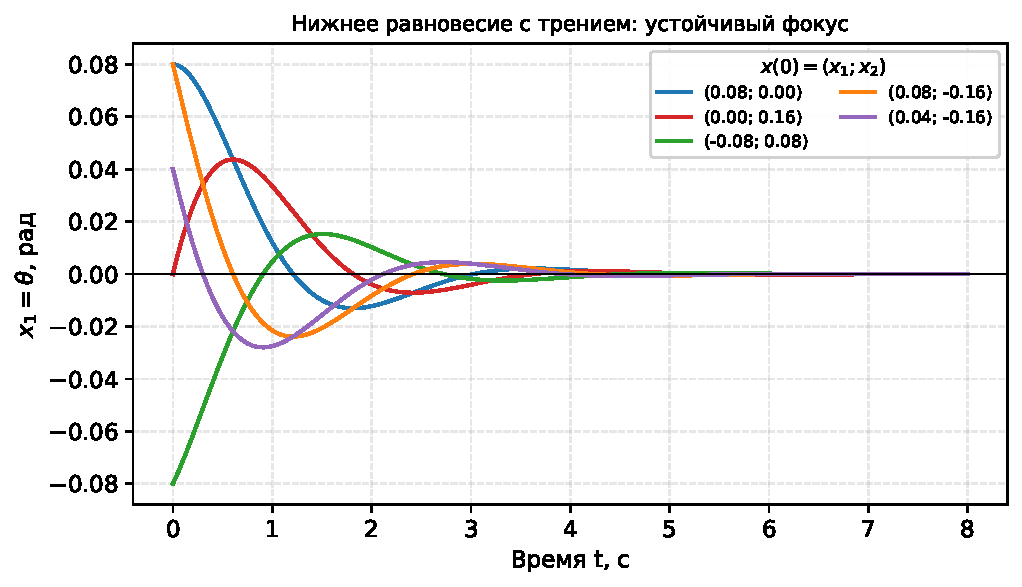
\includegraphics[width=0.82\linewidth]{../figures/t3_2_x1.pdf}
\caption{Затухающие колебания углового отклонения при a=-4, b=-2}\label{fig:t3_2_x1}
\end{figure}

\begin{figure}[H]\centering
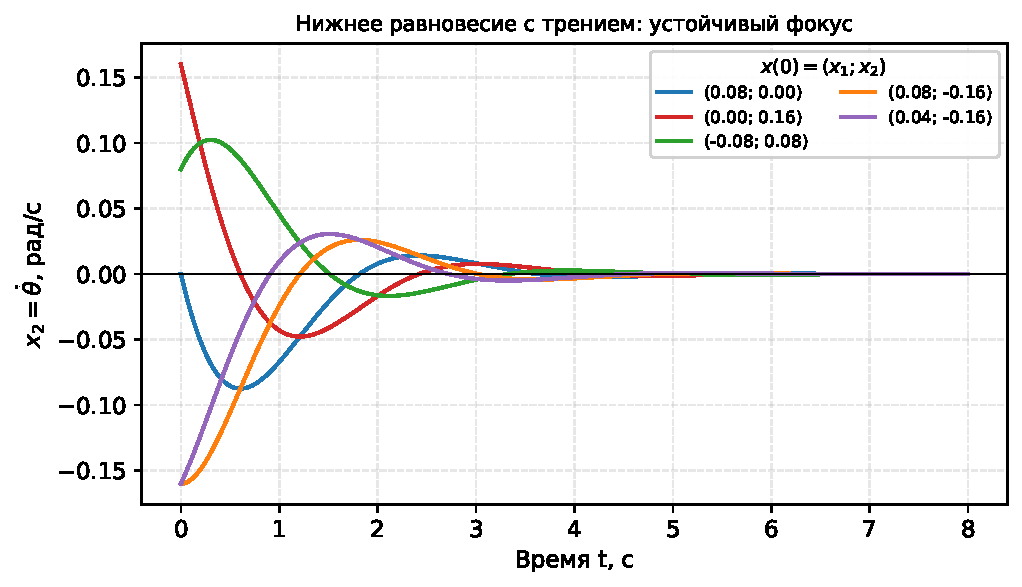
\includegraphics[width=0.82\linewidth]{../figures/t3_2_x2.pdf}
\caption{Затухающие колебания угловой скорости при a=-4, b=-2}\label{fig:t3_2_x2}
\end{figure}

\begin{figure}[H]\centering
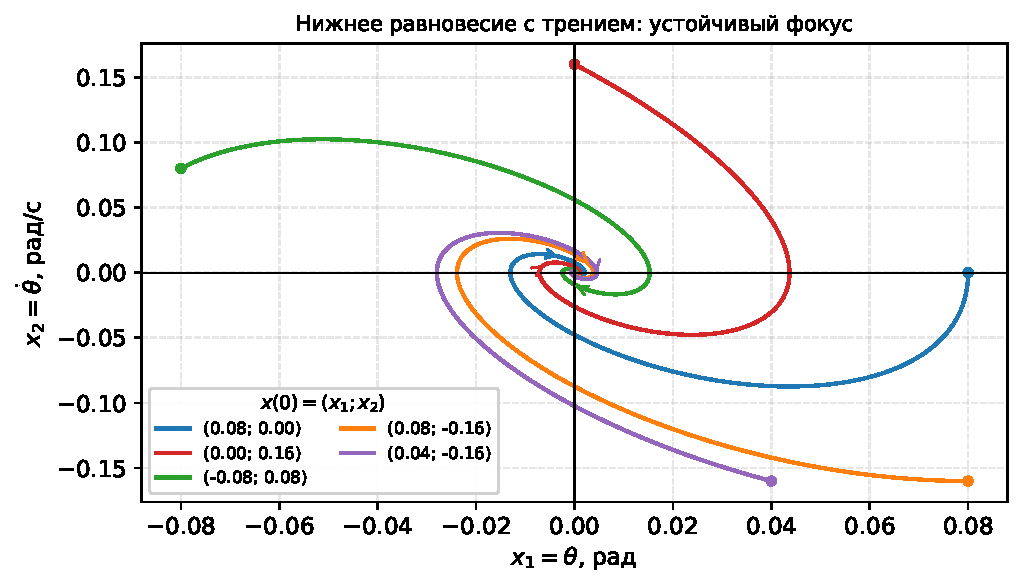
\includegraphics[width=0.82\linewidth]{../figures/t3_2_phase.pdf}
\caption{Фазовые траектории: асимптотически устойчивый фокус}\label{fig:t3_2_phase}
\end{figure}

\textbf{Полная классификация при отрицательных a и b.} Знаки параметров гарантируют асимптотическую устойчивость, но не обязательно колебания. Здесь $\operatorname{tr}A=b<0$, $\det A=-a>0$. Если корни вещественные, их произведение положительно, сумма отрицательна, поэтому оба отрицательные. Если корни комплексные, их вещественные части равны $b/2<0$.

При $D=b^2+4a<0$ получаем устойчивый фокус (затухающие колебания), при $D=0$ — устойчивый вырожденный узел с одним собственным направлением, при $D>0$ — устойчивый узел с двумя собственными направлениями (апериодический режим). Термин «вырожденный узел» здесь относится к кратному собственному числу и одному собственному вектору; матрица обратима.

\subsubsection{Критическое затухание}

Дополнительно берём $a=-4$, $b=-4$, то есть $c=4ml^2$:

\begin{equation}
A_{2c}=\begin{pmatrix}0&1\\-4&-4\end{pmatrix},\qquad
\lambda_{1,2}=-2,\qquad
v=\begin{pmatrix}1\\-2\end{pmatrix},\quad
w=\begin{pmatrix}0\\1\end{pmatrix}.
\end{equation}

Проверка жордановой цепочки: $(A_{2c}+2I)v=0$, $(A_{2c}+2I)w=v$. Собственное подпространство одномерно. Решение:

\begin{equation}
x(t)=e^{-2t}\left[C_1v+C_2(tv+w)\right],\qquad
C_1=q,\quad C_2=u+2q.
\end{equation}

В частности, $x_1(t)=e^{-2t}[q+(u+2q)t]$, $x_2(t)=e^{-2t}[u-2(u+2q)t]$. Множитель $t$ не мешает затуханию: $te^{-2t}\to0$. На рисунках \ref{fig:t3_2c_x1}, \ref{fig:t3_2c_x2}, \ref{fig:t3_2c_phase} показан апериодический переход к нулю, без спирального вращения.

\begin{figure}[H]\centering
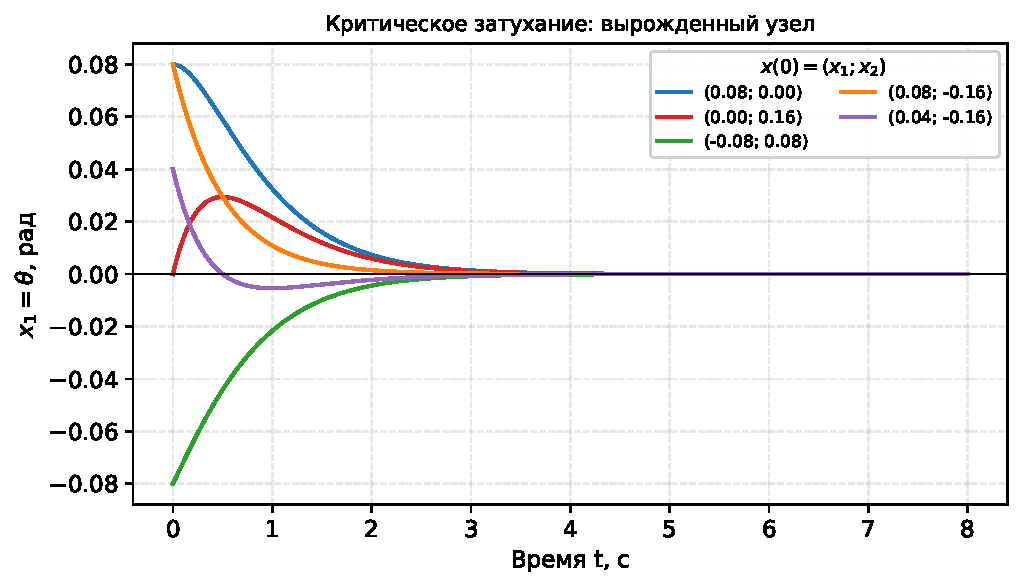
\includegraphics[width=0.82\linewidth]{../figures/t3_2c_x1.pdf}
\caption{Угловое отклонение при критическом затухании}\label{fig:t3_2c_x1}
\end{figure}

\begin{figure}[H]\centering
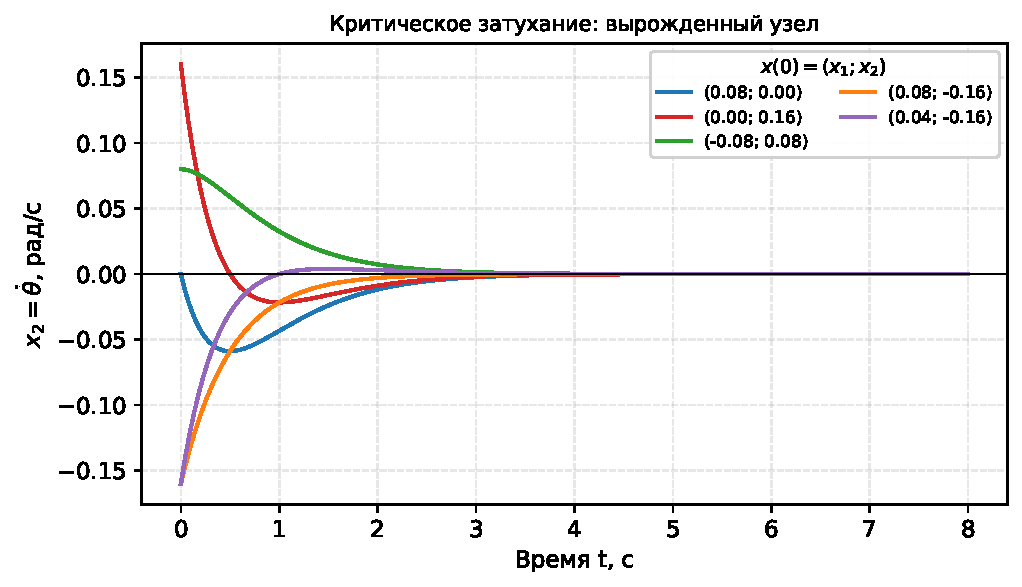
\includegraphics[width=0.82\linewidth]{../figures/t3_2c_x2.pdf}
\caption{Угловая скорость при критическом затухании}\label{fig:t3_2c_x2}
\end{figure}

\begin{figure}[H]\centering
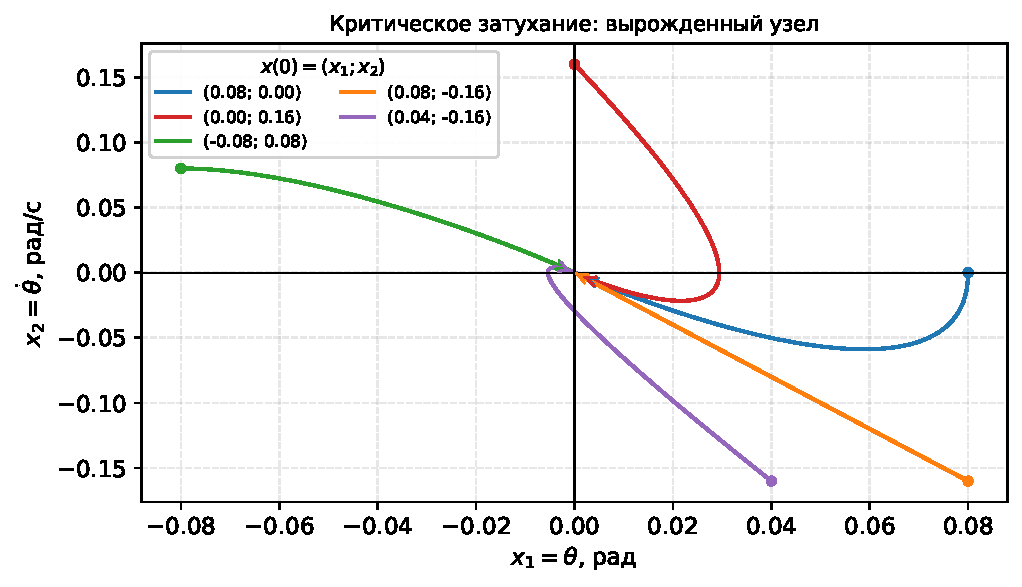
\includegraphics[width=0.82\linewidth]{../figures/t3_2c_phase.pdf}
\caption{Фазовые траектории: устойчивый узел с одной жордановой цепочкой}\label{fig:t3_2c_phase}
\end{figure}

\subsubsection{Сильное затухание}

Берём $a=-4$, $b=-5$, то есть $c=5ml^2$:

\begin{equation}
A_{2o}=\begin{pmatrix}0&1\\-4&-5\end{pmatrix},\quad
\lambda_1=-1,\quad \lambda_2=-4,\quad
v_1=\begin{pmatrix}1\\-1\end{pmatrix},\quad
v_2=\begin{pmatrix}1\\-4\end{pmatrix}.
\end{equation}

Корни различные, обобщённых векторов нет. Решение:

\begin{equation}
x(t)=\frac{u+4q}{3}e^{-t}\begin{pmatrix}1\\-1\end{pmatrix}
-\frac{u+q}{3}e^{-4t}\begin{pmatrix}1\\-4\end{pmatrix}.
\end{equation}

На рисунках \ref{fig:t3_2o_x1}, \ref{fig:t3_2o_x2}, \ref{fig:t3_2o_phase} показан устойчивый узел. Обе моды затухают без периодических колебаний. При ненулевом коэффициенте медленной моды поведение на больших временах определяется $e^{-t}$, поэтому большее сопротивление не гарантирует более быстрое возвращение. Для произвольных начальных скоростей отдельное пересечение равновесия возможно и в апериодическом режиме; отсутствие колебаний не означает монотонность каждой координаты для любых начальных условий.

\begin{figure}[H]\centering
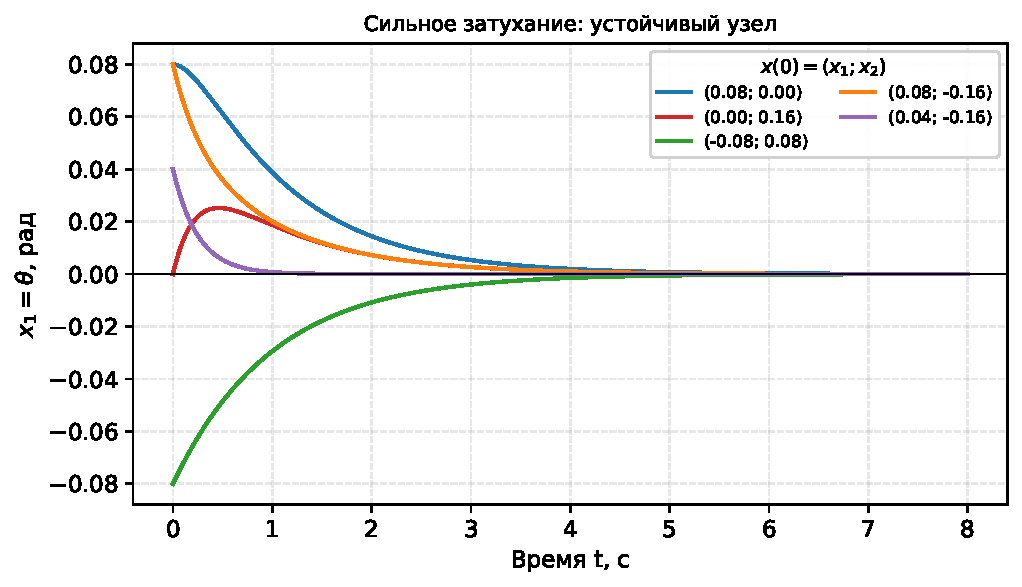
\includegraphics[width=0.82\linewidth]{../figures/t3_2o_x1.pdf}
\caption{Апериодическое угловое отклонение при сильном затухании}\label{fig:t3_2o_x1}
\end{figure}

\begin{figure}[H]\centering
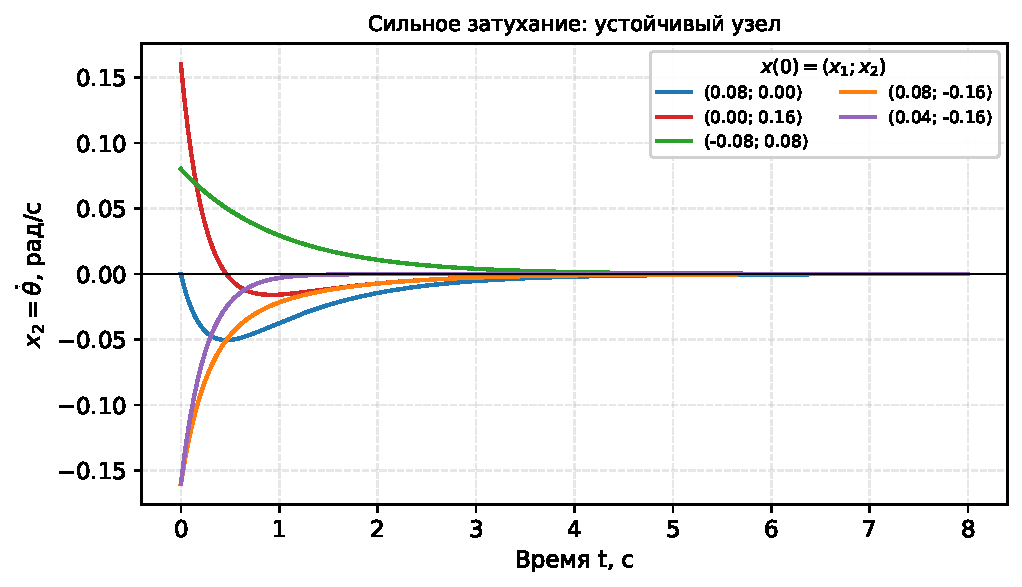
\includegraphics[width=0.82\linewidth]{../figures/t3_2o_x2.pdf}
\caption{Апериодическая угловая скорость при сильном затухании}\label{fig:t3_2o_x2}
\end{figure}

\begin{figure}[H]\centering
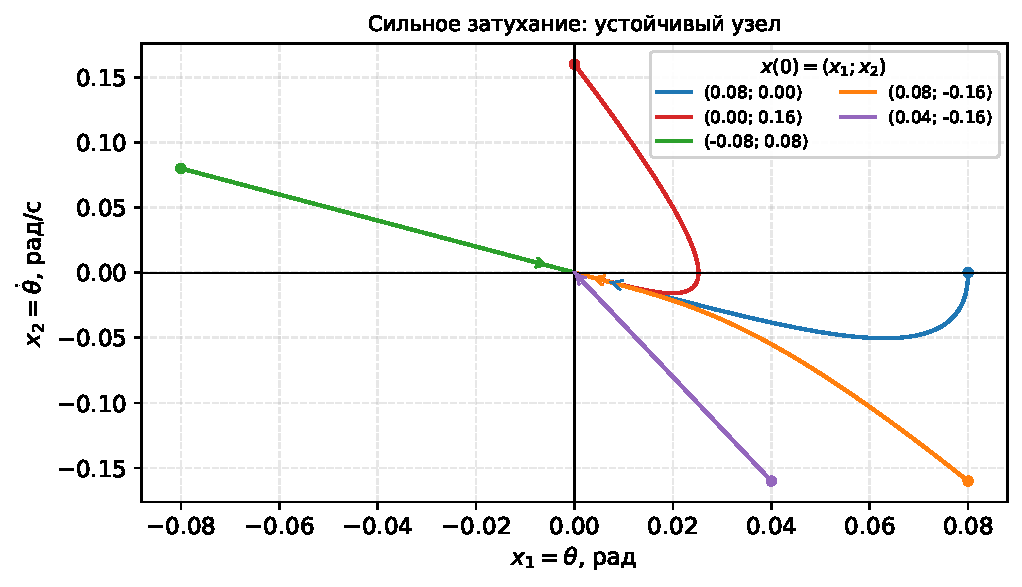
\includegraphics[width=0.82\linewidth]{../figures/t3_2o_phase.pdf}
\caption{Фазовые траектории: устойчивый узел с двумя собственными направлениями}\label{fig:t3_2o_phase}
\end{figure}

\textbf{Вывод.} При $a<0,b<0$ сопротивление рассеивает энергию: $\dot H=bx_2^2\leq0$, где $H=(x_2^2-ax_1^2)/2$ положительно определена. Асимптотическая устойчивость во всех трёх режимах следует из спектра; колебательность определяется дискриминантом. Увеличение сопротивления меняет фокус на критический, а затем на апериодический узел.

\subsection{Случай 3. a > 0, b = 0}

\textbf{Модель.} Маятник на жёстком стержне около верхнего положения без сопротивления. Выбираем $a=4$, $b=0$:

\begin{equation}
A_3=\begin{pmatrix}0&1\\4&0\end{pmatrix},\qquad
\lambda^2-4=0,\qquad \lambda_+=2,\quad\lambda_-=-2,
\end{equation}

\begin{equation}
v_+=\begin{pmatrix}1\\2\end{pmatrix},\qquad
v_-=\begin{pmatrix}1\\-2\end{pmatrix}.
\end{equation}

Обобщённых векторов нет. Решение:

\begin{equation}
x(t)=\frac{2q+u}{4}e^{2t}\begin{pmatrix}1\\2\end{pmatrix}
+\frac{2q-u}{4}e^{-2t}\begin{pmatrix}1\\-2\end{pmatrix}.
\end{equation}

Одна мода растёт, другая затухает, поэтому равновесие неустойчиво, тип портрета — седло. Устойчивая прямая задаётся $x_2=-2x_1$, неустойчивая — $x_2=2x_1$. На общих графиках (рисунки \ref{fig:t3_3_x1}, \ref{fig:t3_3_x2}, \ref{fig:t3_3_phase}) видно расхождение типичных траекторий. Начальное условие $x^{(4)}(0)$ лежит на устойчивой прямой, поэтому для него растущая мода отсутствует.

\begin{figure}[H]\centering
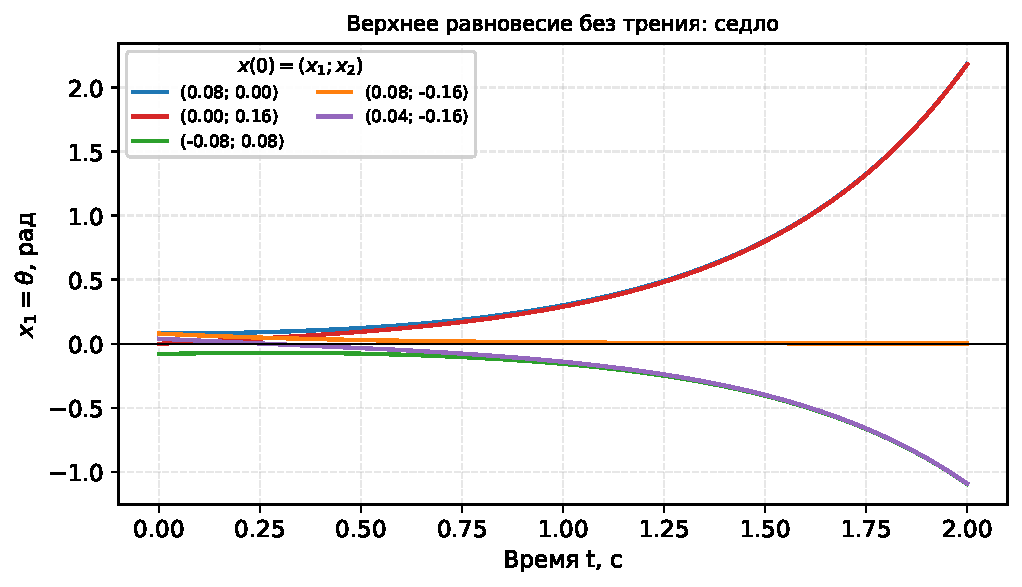
\includegraphics[width=0.82\linewidth]{../figures/t3_3_x1.pdf}
\caption{Угловое отклонение около верхнего положения без сопротивления}\label{fig:t3_3_x1}
\end{figure}

\begin{figure}[H]\centering
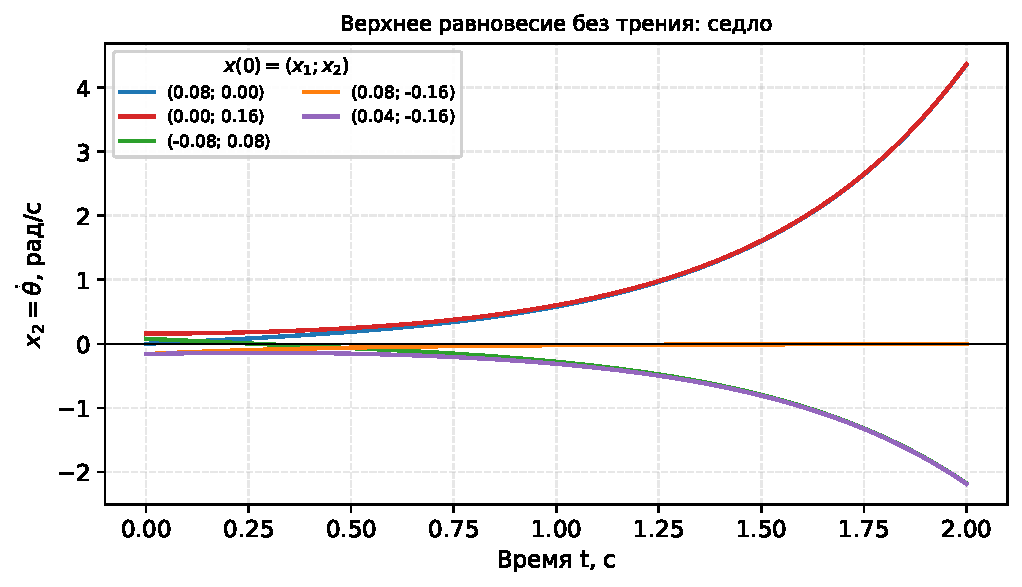
\includegraphics[width=0.82\linewidth]{../figures/t3_3_x2.pdf}
\caption{Угловая скорость около верхнего положения без сопротивления}\label{fig:t3_3_x2}
\end{figure}

\begin{figure}[H]\centering
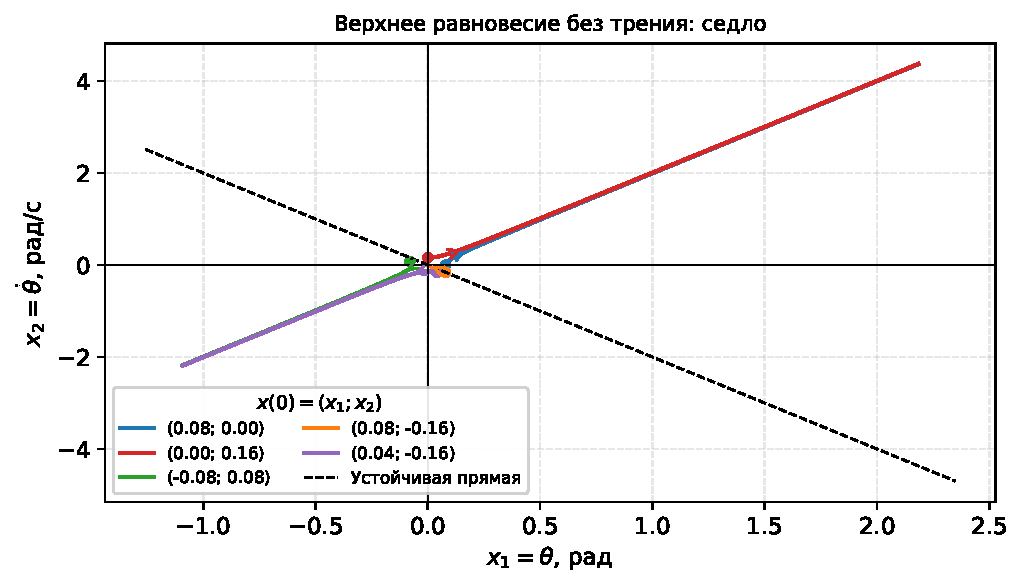
\includegraphics[width=0.82\linewidth]{../figures/t3_3_phase.pdf}
\caption{Фазовые траектории: седло без сопротивления}\label{fig:t3_3_phase}
\end{figure}

Чтобы отдельно показать затухающие движения, выбираем $x(0)=\pm0{,}08v_-$. Тогда $x(t)=\pm0{,}08e^{-2t}v_-$. На рисунках \ref{fig:t3_3_stable_x1}, \ref{fig:t3_3_stable_x2}, \ref{fig:t3_3_stable_phase} обе ветви приближаются к нулю.

\begin{figure}[H]\centering
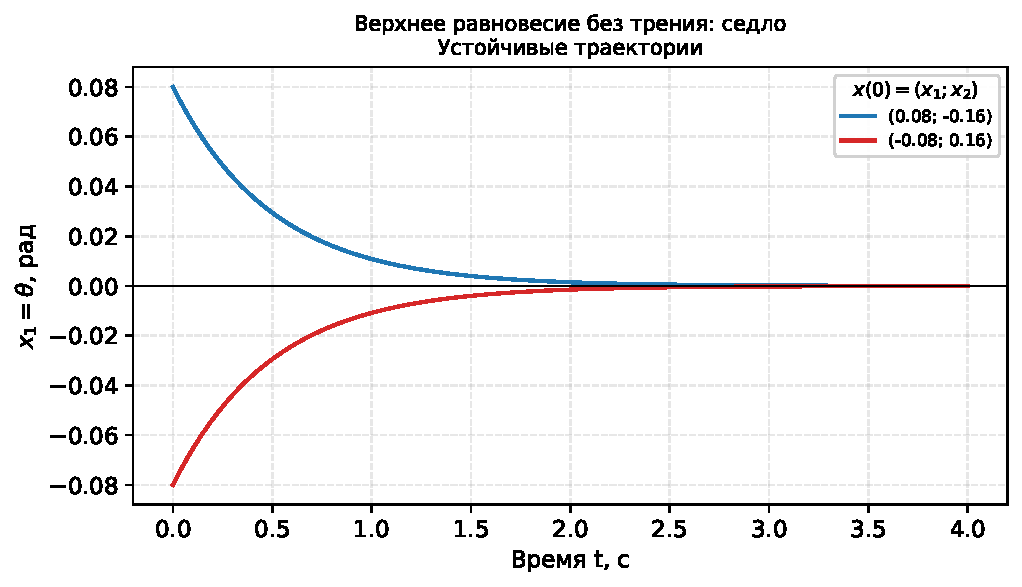
\includegraphics[width=0.82\linewidth]{../figures/t3_3_stable_x1.pdf}
\caption{Устойчивые траектории седла без сопротивления: отклонение}\label{fig:t3_3_stable_x1}
\end{figure}

\begin{figure}[H]\centering
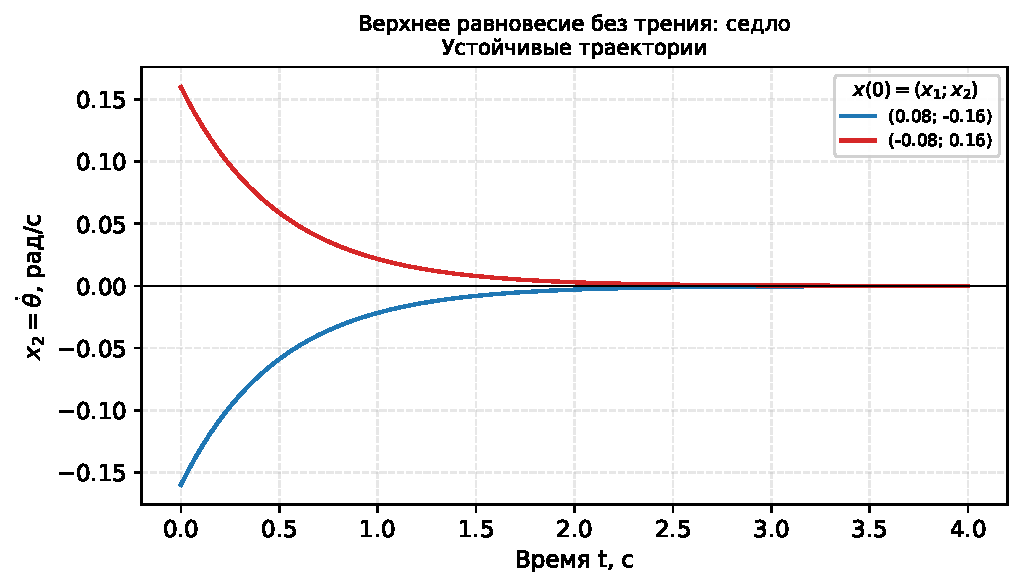
\includegraphics[width=0.82\linewidth]{../figures/t3_3_stable_x2.pdf}
\caption{Устойчивые траектории седла без сопротивления: скорость}\label{fig:t3_3_stable_x2}
\end{figure}

\begin{figure}[H]\centering
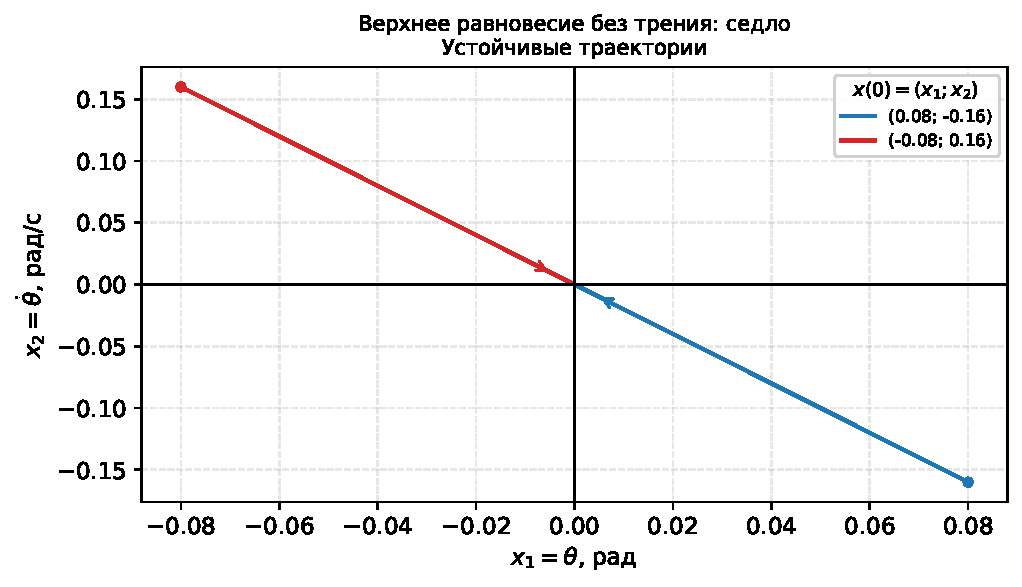
\includegraphics[width=0.82\linewidth]{../figures/t3_3_stable_phase.pdf}
\caption{Устойчивая прямая седла без сопротивления}\label{fig:t3_3_stable_phase}
\end{figure}

\textbf{Вывод.} Существование отдельных решений, стремящихся к нулю, не делает равновесие устойчивым. Любая ненулевая примесь растущей моды $e^{2t}v_+$ приводит к уходу от него. В линейной модели сохранённая величина $(x_2^2-4x_1^2)/2$ не положительно определена, поэтому сохранение такой энергии не обеспечивает устойчивости верхнего положения.

\subsection{Случай 4. a > 0, b < 0}

\textbf{Модель.} Маятник около верхнего положения с вязким сопротивлением. Выбираем $a=4$, $b=-3$, то есть $c=3ml^2$:

\begin{equation}
A_4=\begin{pmatrix}0&1\\4&-3\end{pmatrix},\qquad
\lambda^2+3\lambda-4=(\lambda-1)(\lambda+4),
\end{equation}

\begin{equation}
\lambda_+=1,\quad\lambda_-=-4,\qquad
v_+=\begin{pmatrix}1\\1\end{pmatrix},\quad
v_-=\begin{pmatrix}1\\-4\end{pmatrix}.
\end{equation}

Обобщённых векторов нет. Решение:

\begin{equation}
x(t)=\frac{4q+u}{5}e^t\begin{pmatrix}1\\1\end{pmatrix}
+\frac{q-u}{5}e^{-4t}\begin{pmatrix}1\\-4\end{pmatrix}.
\end{equation}

Равновесие по-прежнему неустойчиво: седло с устойчивой прямой $x_2=-4x_1$ и неустойчивой прямой $x_2=x_1$. В этом случае на устойчивой прямой лежит $x^{(5)}(0)$. На рисунках \ref{fig:t3_4_x1}, \ref{fig:t3_4_x2}, \ref{fig:t3_4_phase} типичные решения расходятся, хотя медленнее, чем в случае 3.

\begin{figure}[H]\centering
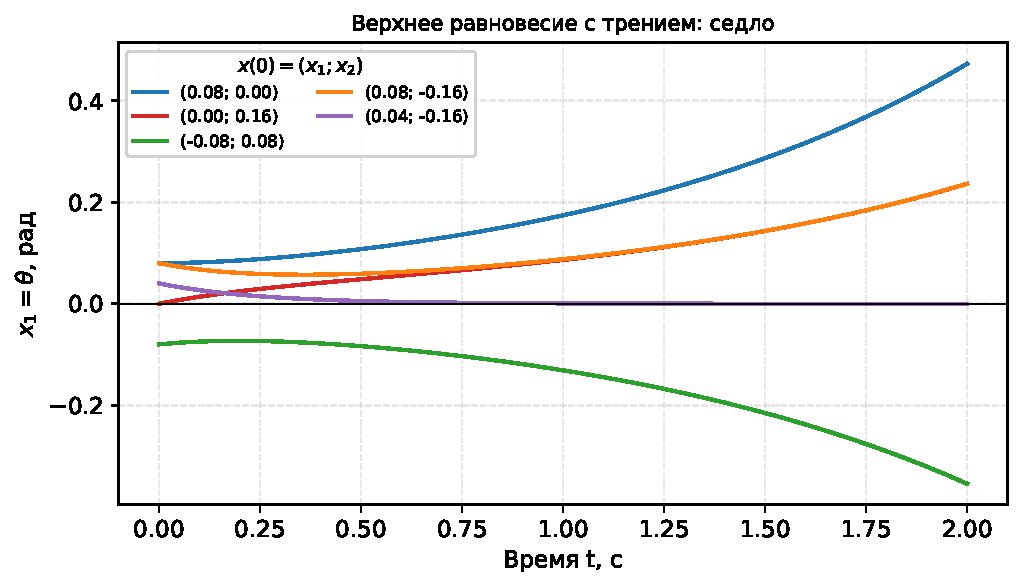
\includegraphics[width=0.82\linewidth]{../figures/t3_4_x1.pdf}
\caption{Угловое отклонение около верхнего положения с сопротивлением}\label{fig:t3_4_x1}
\end{figure}

\begin{figure}[H]\centering
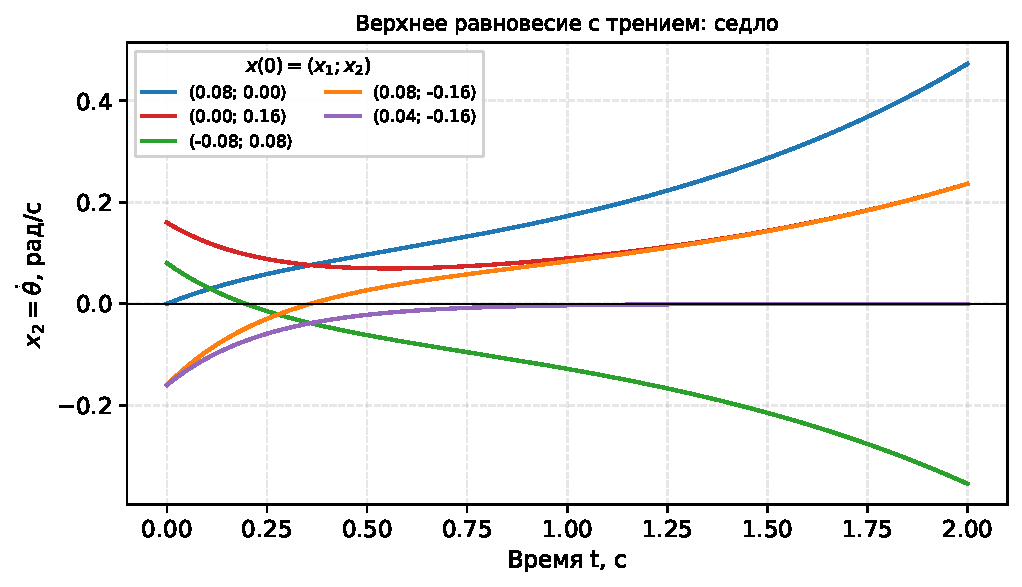
\includegraphics[width=0.82\linewidth]{../figures/t3_4_x2.pdf}
\caption{Угловая скорость около верхнего положения с сопротивлением}\label{fig:t3_4_x2}
\end{figure}

\begin{figure}[H]\centering
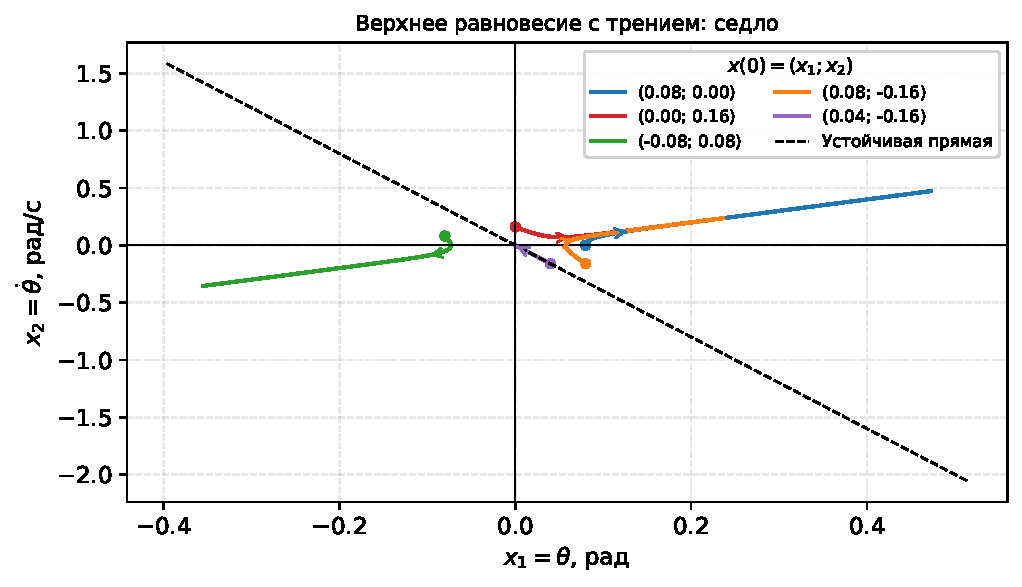
\includegraphics[width=0.82\linewidth]{../figures/t3_4_phase.pdf}
\caption{Фазовые траектории: седло с сопротивлением}\label{fig:t3_4_phase}
\end{figure}

Отдельно берём $x(0)=\pm0{,}08v_-$. Решения $x(t)=\pm0{,}08e^{-4t}v_-$ показаны на рисунках \ref{fig:t3_4_stable_x1}, \ref{fig:t3_4_stable_x2}, \ref{fig:t3_4_stable_phase}. Они стремятся к нулю быстрее, чем устойчивые решения в случае 3.

\begin{figure}[H]\centering
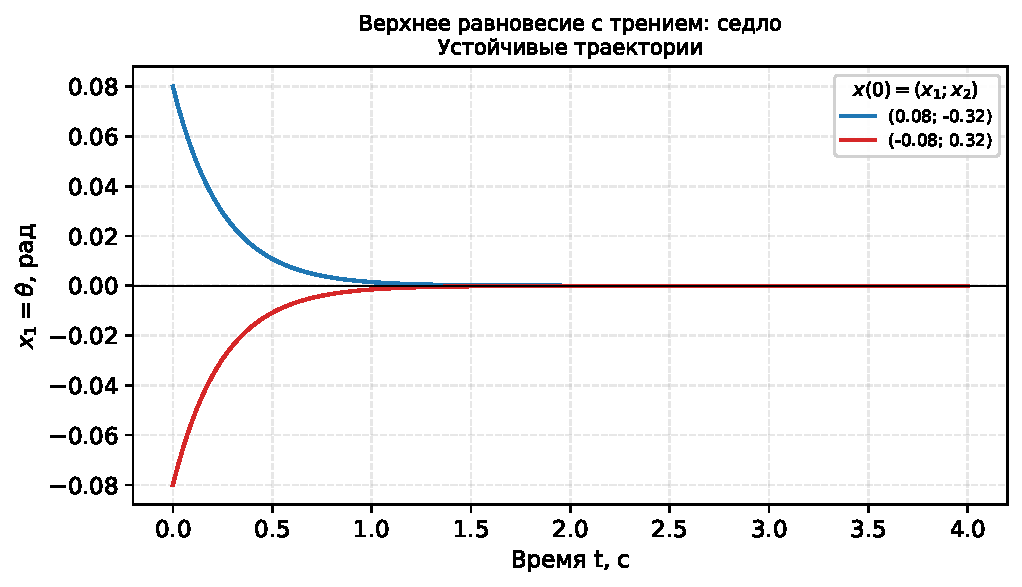
\includegraphics[width=0.82\linewidth]{../figures/t3_4_stable_x1.pdf}
\caption{Устойчивые траектории седла с сопротивлением: отклонение}\label{fig:t3_4_stable_x1}
\end{figure}

\begin{figure}[H]\centering
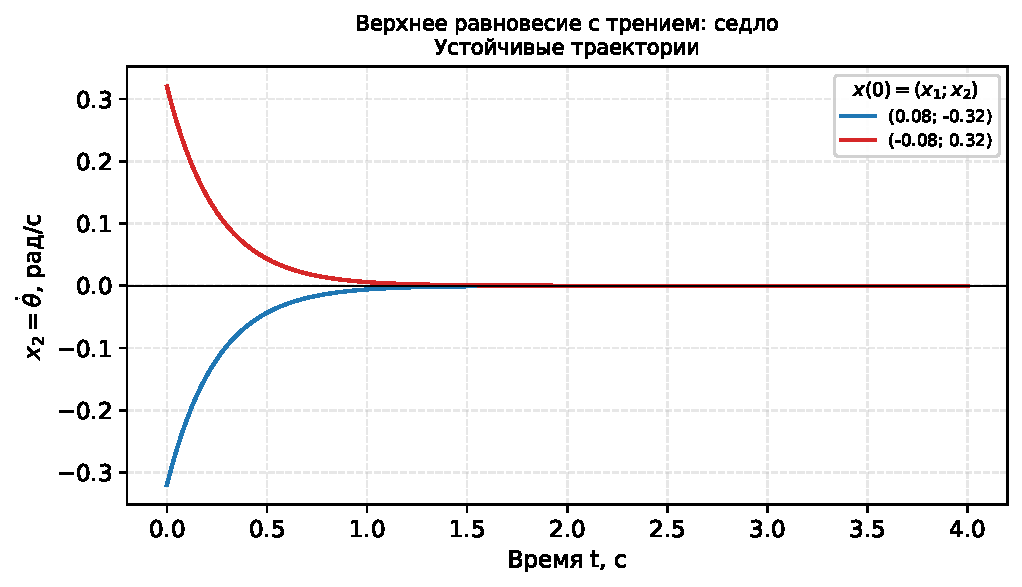
\includegraphics[width=0.82\linewidth]{../figures/t3_4_stable_x2.pdf}
\caption{Устойчивые траектории седла с сопротивлением: скорость}\label{fig:t3_4_stable_x2}
\end{figure}

\begin{figure}[H]\centering
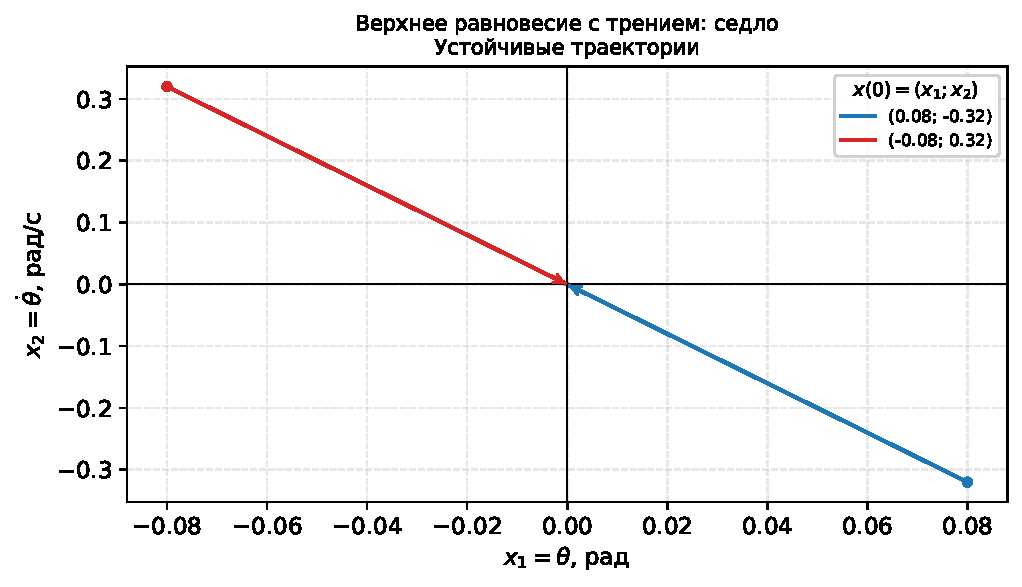
\includegraphics[width=0.82\linewidth]{../figures/t3_4_stable_phase.pdf}
\caption{Устойчивая прямая седла с сопротивлением}\label{fig:t3_4_stable_phase}
\end{figure}

\textbf{Вывод.} Вязкое сопротивление замедляет падение из верхнего положения, но само по себе не стабилизирует его. Для любого $a>0$ произведение собственных чисел равно $-a<0$, поэтому корни вещественные и имеют разные знаки независимо от отрицательного $b$. Более явно, $\sqrt{b^2+4a}>|b|$, так что $\lambda_+>0$. Чтобы стабилизировать верхнее положение, требуется изменить эффективное возвращающее действие, например управлением, а одного пассивного демпфера недостаточно.

\subsection{Итог по заданию 3}

При $a<0$ действует возвращающая сила: без сопротивления возникает центр, с положительным физическим сопротивлением — асимптотически устойчивый фокус либо узел. При $a>0$ сила уводит систему от равновесия: в обоих рассмотренных случаях возникает седло. Отрицательный $b$ рассеивает энергию, однако не устраняет положительное собственное число при $a>0$.

Для комплексных различных и вещественных различных корней достаточно собственных векторов $(1,\lambda)^T$. Обобщённый вектор потребовался только для критического затухания с кратным корнем. Результаты моделирования согласуются с аналитическими решениями; графики иллюстрируют спектральную классификацию, а не заменяют доказательство устойчивости.

\subsection{Воспроизведение}

Из корня репозитория: \texttt{python3 labs/lab04/code/task3.py}. Нужны NumPy и Matplotlib. Скрипт создаёт отдельные PDF и PNG для каждой координаты и фазового портрета, данные в NPZ и сводку в JSON. Численная проверка: \texttt{python3 labs/lab04/verification/check\_task3.py} (дополнительно нужны SciPy и SymPy).
